\chapter{Theoretical Framework}
\label{ch:marco}
This section presents concepts and academic works that form the theoretical foundation of the document.
Special attention is given to normative documents and state-of-the-art MBSE research that characterize the needs, requirements, interfaces and technical criteria of nanosatellite EPS, as per the first objective of the project.

\section{NASA engineering lifecycle}
The NASA reference lifecycle progresses from Pre-Phase A (Concept Studies), through A (Concept and Technology Development) and B (Preliminary Design and Technology Completion), to C (Final Design and Fabrication). Requirements, design and technical management processes recur as products mature. Phase C normally includes detailed design, hardware fabrication and software coding. CDR occurs during C before deliverable coding. SIR occurs at its end to assess integration readiness \citep[Secs.~2.2--2.3, 3.3--3.6 and Table~6.7-1]{nasa2016systems}.

\section{Concept of Operations}
A Concept of Operations is a high-level description of how a system will be used to meet stakeholder expectations, usually in a time sequence. It provides an operational perspective that guides requirements and architecture development \citep[Sec.~4.1.1.2.4 and Appendix~B]{nasa2016systems}.

\section{Verification and validation}
Verification establishes conformity to applicable requirements. Validation assesses suitability for stakeholder expectations and ConOps in the intended environment. Validation may use models under representative simulated conditions. Analysis is a valid validation method. Requirements validation also checks correctness, feasibility, consistency, verifiability and stakeholder suitability. Model calibration adjusts parameters against data. Independent validation data, assumptions, uncertainty and the intended validity domain are needed to assess a model's credibility \citep[Secs.~2.4, 4.2 and~5.3--5.4]{nasa2016systems}\citep[pp.~7--9]{handpicked-0001}.

\section{Model-based Systems Engineering}
Buruso et al. describe model-based systems engineering (MBSE) as the use of a shared system model across engineering disciplines and throughout the system lifecycle, from identifying stakeholder needs to development and operations \cite{buruso2026modelbased}.
Such models can capture functional, logical, and physical characteristics at different levels of design detail.
They can also support simulation, comparison of candidate solutions, and data exchange across tools and engineering roles \cite{buruso2026modelbased}.
Potential benefits of the adoption of MBSE include lower documentation effort and development cost, better system understanding and collaboration, earlier fault detection, and reduced technical risk \cite{buruso2026modelbased}.

\section{The Object-Oriented Systems Engineering Methodology}
OOSEM is a top-down, scenario-driven MBSE method that serves to analyze, specify, design, and support the verification of systems. Its primary output is an integrated system model with consistent views of behavior, structure, properties, and requirements traceability. Its specification and design activities progress from stakeholder needs and black-box system requirements to logical and physical architectures. Engineering analysis, trade studies, and traceability span these activities. The activities are tailored and iterated rather than executed as fixed sequential phases \citep{friedenthal2014practical}.

Figure~\ref{fig:systems-engineering-technical-processes} summarizes the systems engineering technical process. Stakeholder needs inform system specification and design. Component requirements guide component design, implementation, and test. Verified components feed system integration and test. Feedback from component work and integration returns to system specification and design \citep[Fig.~1.1]{friedenthal2014practical}. OOSEM implements system specification and design and supports integration and verification through model-based test cases. The development process can be applied recursively at successive levels of the system hierarchy \citep[Sec.~17.1.2]{friedenthal2014practical}.

\begin{figure}[htbp]
    \centering
    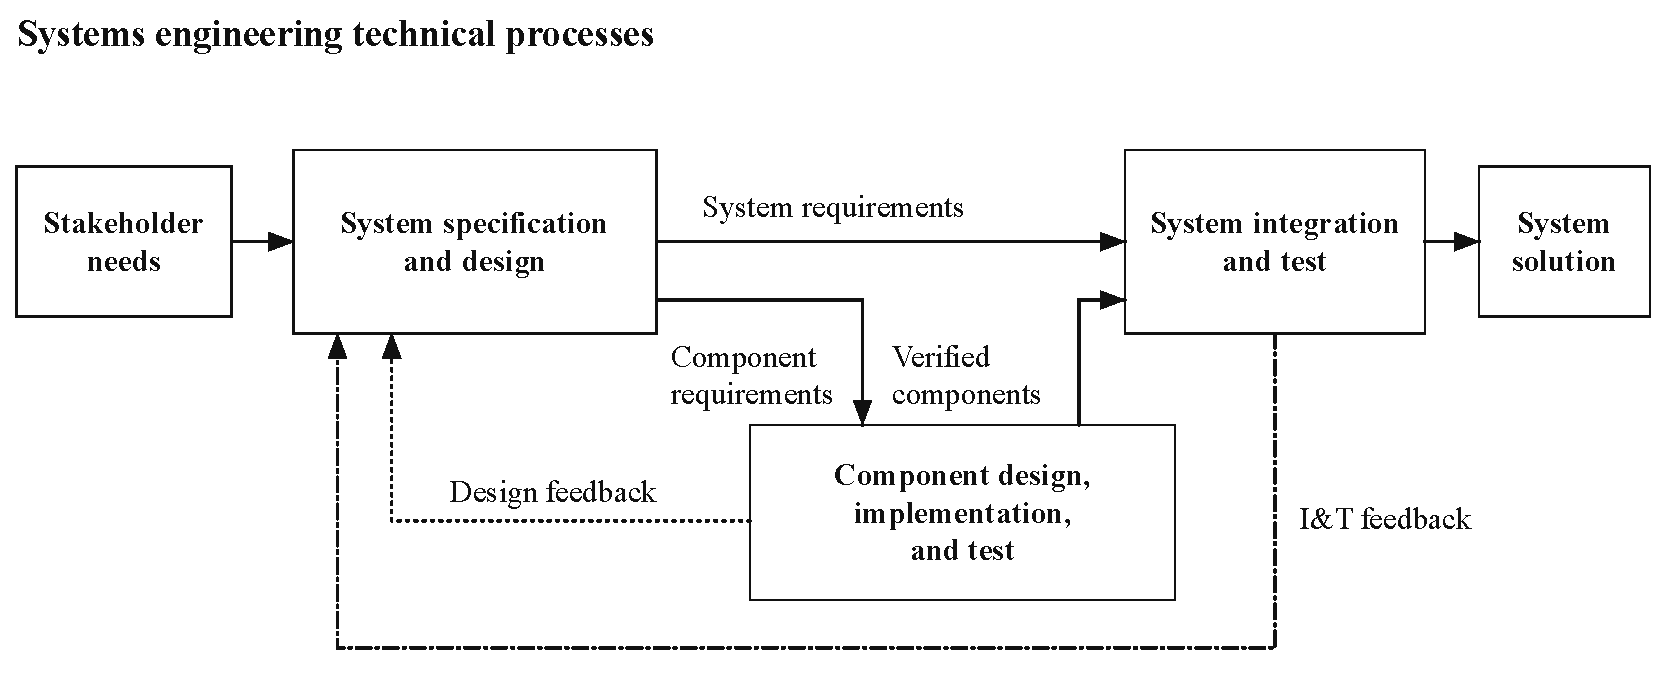
\includegraphics[width=\linewidth]{fig/systems-engineering-technical-processes.pdf}
    \caption[Simplified systems engineering technical processes.]{Simplified systems engineering technical processes. Solid arrows carry forward exchanges. Dotted arrows carry design feedback. Dash-dot arrows carry integration and test feedback. Adapted from \citet[Fig.~1.1]{friedenthal2014practical}.}
    \label{fig:systems-engineering-technical-processes}
\end{figure}

\section{Stakeholders.}
In OOSEM, a stakeholder is a person or organization with an interest in the system across its lifecycle. A stakeholder role identifies whose concerns must be addressed \citep[Secs.~17.3.2 and 17.3.5]{friedenthal2014practical}.

\section{Operational domain as-is and to-be, and enterprise.}
An operational domain provides the context for the system of interest. It contains the operational system, the users and external systems with which it interacts, and the relevant environment. An as-is domain characterizes the current context sufficiently to understand stakeholder concerns. A to-be domain describes the intended context after the mission need is addressed. Within a domain, an enterprise is an aggregation of systems and users that collaborate to achieve a set of mission objectives. It contains the system of interest and the supporting participants needed to accomplish those objectives, while other actors and environmental elements may remain external to it \citep[Sec.~17.3.2]{friedenthal2014practical}.

\section{Normative documents applicable to CUBICS proposal}
The basic normative references are the CUBICS announcements of opportunity, first released in 2022 and most recently in 2026 \citep{csa2022cubics,csa2026cubics}.
These documents define proposal eligibility and the evaluation process used to select recipients of CSA funding \citep[Secs.~3 and~5]{csa2026cubics}.
The 2022 call specified design and test reviews adapted from the NASA Systems Engineering Handbook for college and university payload or CubeSat projects \citep[App.~B.7]{csa2022cubics}. The 2026 call allows flexibility in development strategies while evaluating the documented project plan, milestones and schedule \citep[FAQ~24 and App.~C.2.1]{csa2026cubics}.
The Canadian Space Agency also published the Systems Engineering Mission Tailoring Guidelines (CSA-SE-GDL-0001), which provide guidance on tailoring systems engineering requirements by mission class, particularly for smaller Class D missions like academic nanosatellites and personnel training \citep[Secs.~1.1--1.3]{csa2020tailoring}.

By applying CSA-SE-GDL-0001 to the NASA systems engineering lifecycle, a mission treated as CSA Class D can retain the progression from concept studies through design, fabrication, integration, operations and closeout.
Engineering effort is scaled to the mission's objectives, resources and accepted risk of mission failure \citep[Secs.~3 and~3.11]{nasa2016systems}\citep[Sec.~3.2]{csa2020tailoring}.
Plans can be consolidated into a concise project plan while retaining essential requirements, interfaces, resource budgets, risks and verification evidence \citep[Sec.~3.11.4]{nasa2016systems}\citep[Secs.~4.2--4.4 and App.~B]{csa2020tailoring}.

Class D design assurance can favor commercial components, limited redundancy and fewer separate physical development and qualification units where the consequences of failure permit.
Frequent engineering discussions and peer reviews provide oversight, supported by recorded tailoring decisions, residual risks and required approvals \citep[Sec.~3.4.1]{csa2020tailoring}\citep[Sec.~3.11.3]{nasa2016systems}.

Normative documents provide requirements directly applicable to the EPS \citep[Sec.~2.3]{calpoly2022cds}.
They also constrain other subsystems, whose interfaces and operating needs lead to derived EPS requirements \citep[Secs.~4.2--4.3]{nasa2016systems}.
United Nations guidance and United States regulations provide comparative references for battery safety, passivation and disposal \citep{unoosa2010debris,fcc2026satellitecommunications}.
Canadian licensing requires five-year disposal and at least 90\% probability of disposal success \citep[Decisions~D10--D11]{ised2026debris}.

\section{Generic models of EPS requirements and architecture}
The CubeSat Design Specification and EXOpod Nova manual provide preliminary guidance on power isolation, inhibits and charging access \citep{calpoly2022cds,exolaunch2024exopodnova}.
Other subsystems contribute derived EPS requirements through their supply voltages, power consumption and operating schedules \citep[Secs.~2--4]{handpicked-0003}\citep[Sec.~2]{review-0289}.

The Object Management Group's CSRM Profile 1.1 specification complements these engineering sources with standardized categories for mission, spacecraft, subsystem and component requirements \citep[Sec.~6.1]{omg2025csrm}.
It relates requirements to the architectural elements that satisfy them and to verification activities with recorded outcomes \citep[Secs.~6.3--6.4]{omg2025csrm}.
These relationships support tracing normative and derived EPS requirements through design and verification.
The surveyed literature identifies it as mature, with 18 papers in its core research lineage covering the Radio Aurora Explorer predecessors, reference model development, and companion methods for behavior, technical measurement, validation and mission engineering \citep{review-1646,review-1621,review-1554,review-1563,review-1494,review-1487,review-1451,review-1446,kaslow2017status3,kaslow2017behaviors,kaslow2018verification,review-1288,kaslow2018status4,kaslow2019csrm,kaslow2020csrm,review-1051,kaslow2022mission,rudder2026metamodel}.

\section{Generic models of EPS components}
Luccisano et al. model shared component identity, manufacturer, mass, power by operating mode and margins per component. Their distinction between aggregate and detailed component budgets supports explicit accounting boundaries \citep[Secs.~3.1--3.2]{luccisano2024formalization}. Ceglarek and Bertrand contribute a catalog built from manufacturer datasheets with controlled parameter meanings and units. Their experience with inconsistent datasheets motivates retaining the original value and its reviewed interpretation \citep[Sec.~3]{review-0257}. The proposed schema will extend these contributions with source revisions, operating conditions, uncertainty, supported configurations and interface descriptions. These extensions will make catalog comparisons assessable.

El Hachimi et al. supply the solar maximum power point and EOL properties, battery energy and cycle-life criteria, and examples of named cells and their arrangements \citep[Secs.~3 and~6.2]{handpicked-0003}. Casado et al. contribute solar current--voltage curves with irradiance and temperature conditions, battery discharge curves and internal resistance \citep[Secs.~2.1 and~2.3]{review-0573}. Boan contributes the series/parallel configuration and mission illumination needed to assess a selected assembly \citep[Sec.~3]{review-0289}. These sources motivate separate cell and assembly records, conditional electrical characteristics and installation geometry. Wijaya et al. contribute fixed commercial product properties alongside sized alternatives. Purchased panels and packs will retain their specified dimensions, mass and ratings \citep[Sec.~III.A--B, Appendix]{review-0145}.

El Hachimi et al. contribute conditioning and bus alternatives, converter input compatibility, independently controlled outputs, protection thresholds, timing and autonomous protection functions \citep[Secs.~4 and~7.1--7.6]{handpicked-0003}. Casado et al. contribute regulator operating modes and transitions, protected output rails, and distribution efficiency estimates based on measurements \citep[Secs.~2.2 and~2.4]{review-0573}. The models will therefore distinguish conversion capabilities, electrical operating limits, loss data, channel organization and protection behavior. A controller integrated circuit record will retain its required external circuit. Its ratings alone will establish no complete converter or protected output.

In complementary approach, digital twin research supports obtaining verification evidence without fabricating the complete EPS.
Casado et al. use models validated against physical measurements to simulate EPS behavior over a complete orbital cycle \citep[Secs.~3--4]{review-0573}.
Related battery digital twin work by Zhu et al. (2025) describes virtual testing and software-in-the-loop verification without physical prototypes, followed by hardware-in-the-loop testing \citep[p.~3]{handpicked-0001}.
This is consistent with the tailored lifecycle, since NASA recognizes modeling and simulation as verification by analysis and recommends selecting methods according to project constraints and accepted risk \citep[Sec.~5.3.1.2]{nasa2016systems}.
The CSRM specification likewise includes verification under simulated or modeled conditions within its definition of analysis \citep[Sec.~6.6.8]{omg2025csrm}.
Selected requirements can therefore be verified before fabrication using credible models, while retaining the physical safety and qualification tests required by the mission and launcher \citep[Sec.~5.3.1.2]{nasa2016systems}\citep[Secs.~2.3 and~3]{calpoly2022cds}.

\section{EPS development lifecycle}
EPS development workflows link mission inputs and power budgeting to architecture, design, integration and verification within the spacecraft lifecycle \citep{handpicked-0003,review-0289}.
These workflows can be understood as an EPS development lifecycle embedded within the tailored spacecraft lifecycle, progressing from applicable normative and derived requirements to a design validated against them.
El Hachimi et al. cover the progression through functional and environmental qualification, while Boan demonstrates the preliminary stages through iterative sizing and energy balance simulations \citep[Secs.~2--5]{handpicked-0003}\citep[Secs.~2--4]{review-0289}.

Analysis of system models provides verification evidence during preliminary design.
Strobbe et al. link an EPS MBSE model to power budget calculations and propagate parameter changes to identify violated requirement constraints \citep[Secs.~III--IV]{review-0764}.
Jbara automates power and other spacecraft budget calculations and accepts or rejects candidate component selections against numerical limits \citep[Secs.~4--5]{review-0270}.
Wijaya et al. generate alternative architectures, couple subsystem sizing calculations and compare their mass, power and dimensional results with mission requirements \citep[Sec.~5.2]{review-0055}.
Their simplified sizing models support preliminary trends and relative trade-offs \citep[Sec.~6.1]{review-0055}.
